\documentclass[tikz,border=6pt]{standalone}
\usepackage{amsmath}
\usepackage{xcolor}

\definecolor{blockblue}{HTML}{4A90D9}

\begin{document}
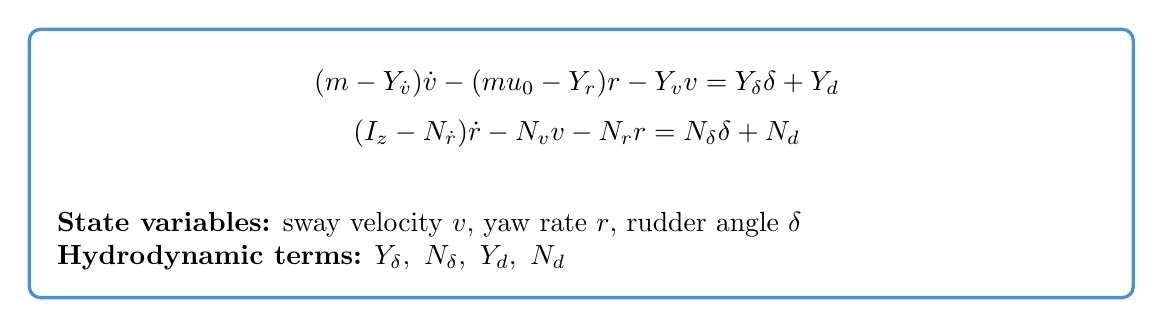
\begin{tikzpicture}[line width=1.2pt]
  \node[
    draw=blockblue,
    rounded corners=4pt,
    inner sep=10pt,
    align=left
  ] at (0,0) {
    \begin{minipage}{13.2cm}
    \[
    (m-Y_{\dot v})\dot v-(m u_0-Y_r)r-Y_v v = Y_\delta \delta + Y_d
    \]
    \[
    (I_z-N_{\dot r})\dot r-N_v v-N_r r = N_\delta \delta + N_d
    \]
    \vspace{3pt}

    \textbf{State variables:}
    sway velocity $v$, yaw rate $r$, rudder angle $\delta$ \\
    \textbf{Hydrodynamic terms:}
    $Y_\delta,\ N_\delta,\ Y_d,\ N_d$
    \end{minipage}
  };
\end{tikzpicture}
\end{document}
